\documentclass[11pt,openany]{book}
\usepackage{zpj}
\usepackage{ulem}
\usepackage{fancyvrb}
\usepackage[linkcolor=blue,citecolor=blue,urlcolor=blue]{hyperref}
\definecolor{codec}{RGB}{100,64,0}
\definecolor{dgreen}{HTML}{005545}
\newcommand{\command}[1]{\texttt{\textcolor{codec}{#1}}}
\newcommand{\zy}{zypper或YaST}
\newcommand{\soft}[1]{\texttt{\textcolor{dgreen}{#1}}}
\newcommand{\simp}[2]{\command{#1}$=$\command{#2}}
\newcommand{\menu}[1]{\fbox{#1}}
\newcommand{\me}{$\rightarrow$}
\newcommand{\emp}[1]{\textbf{#1}}
\begin{document}
\title{openSUSE新手指南}
%\author{朱沛俊\thanks{我的邮箱:\href{mailto:zpj.ustc@gmail.com}{zpj.ustc@gmail.com}}}
\author{\href{mailto:zpj.ustc@gmail.com}{\texttt{zpj.ustc}}}
\maketitle
\chapter*{关于}
%请不要修改这个文件,这个文件是make自动生成
身边有很多同学想学习或者需要使用Linux,然而最初从Windows转到Linux的人往往有各种不习惯,遇到很多问题。

这个指南就是一个简要的入门教程,尽量使得新手学会Linux/openSUSE下的一些基本知识,通过阅读或查阅本文档就能够解决一些常见的问题,以便于能够专心工作,而不是为一个操作系统操碎了心。
%请不要修改这个文件,这个文件是make自动生成


本文档源文档现已托管在\href{https://github.com/zpj-ustc/openSUSE-novice-guide}{Github}上,欢迎对其进行修改分发。
\newpage
\tableofcontents
\newpage


\chapter{基础部分}
让你折腾完了你就得到了一个勉强能用的openSUSE
\section{安装openSUSE以及分区}
安装openSUSE请参见\href{https://zh.opensuse.org/%E6%96%B0%E6%89%8B%E6%9D%91}{新手村}。
另外本文主要针对安装了KDE桌面环境的openSUSE的用户,其他环境如GNOME下可能会有某些地方不同。

对于桌面用户,一般只需要\command{/, /home, swap}三个分区即可,分区大小与具体使用有关。\command{swap}的大小一般桌面用户可以用公式$y=2\sqrt{x}$计算,其中$y$代表\command{swap}分区的大小,$x$代表内存大小,单位皆为G。而\command{/home}大小较为随意,最好不小于50G。根分区\command{/}则主要取决于你安装的程序(它们会在\command{/usr}中),比如你安装了\textsc{Matlab}就会占用7.9G,而Mathematica 会占用约4.5G,如果你将要安装这类大型软件,建议至少应该有60G的根分区空间。分区大小并没有严格的准则。
如果可能的话,为每个文件系统至少保留$25\%$的额外空间以应对今后的变化,还可以避免文件系统碎片。

对于密码,不要设的太复杂,不然每次安装软件都输一次密码将会很痛苦。当然,密码也是可以之后再修改的。
\section{基本概念}
\subsection{Linux的一些基本概念}
\paragraph{终端} Shell是各种命令的入口,而终端相当于是为Shell提供了一个图形界面,如KDE下面的\soft{konsole}。\emp{本文中大部分命令都是在终端中运行的。}

\paragraph{root权限} 顾名思义,root权限就是最根本权限。也就是说,有了root权限,你基本上有了做任何事的权力。
而执行某些命令,如安装、卸载软件包时需要root权限。此时你需要在命令前加sudo才能执行。
默认情况下输入密码时不会有类似于\command{****}的提示符。你也可以用su这个命令切换到root用户,
但是安全起见,在不必要的时候还是不要用su切换到root。注意,在以root运行相关图形程序,需要使用\command{kdesu}来代替\command{sudo}!

\paragraph{软件源} 软件源就是软件下载的来源。如果你已经添加的所有源里面都没有想要的软件包,但是在软
件包搜索或其他源中有,那你只需添加相应的源,再刷新源即可在\zy 中找到。添加软件源的方法可以参见\href{https://zh.opensuse.org/SDB:%E6%B7%BB%E5%8A%A0%E8%BD%AF%E4%BB%B6%E6%BA%90}{添加软件源}
%\item[依赖关系]
\subsection[包管理器]{openSUSE下的包管理器}
openSUSE下安装软件一般先用\zy 搜索,找到了便可以直接用\zy 安装。
如果搜索不到,说明你添加的的所有软件源里面都没有包含这个软件,此时你就需要用软件包搜索了。搜到了便一键安装,否则便只能采取最后方法——自行编译了。如果你你有打包能力并且这个程序不违反OBS相关规定,那么你就把它丢到OBS上面去,
然后别人也可以用这个打好了的包了。
\paragraph{zypper}\label{pre} 它是一个命令行的包管理器,常用命令有
\begin{Verbatim}[formatcom=\color{codec}]
    zypper update #升级软件包
    zypper refresh #刷新软件源
    zypper install PKG1 PKG2 #安装PKG1和PKG2等软件包
    zypper remove PKG1 PKG2 #移除PKG1和PKG2等软件包
\end{Verbatim}
其中上述选项都可以简化输入,对应关系为:
\begin{compactitem}
 \item \simp{update}{up}
 \item \simp{refresh}{ref}
 \item \simp{install}{in}
 \item \simp{remove}{rm}
\end{compactitem}

想要了解更多命令及其选项可以用\command{zypper --help}查看相关帮助。如果不想每次运行\zy (比如搜索软件包)的时候都自动刷新一次,你可以禁用所有软件源的自动刷新:
\begin{Verbatim}[formatcom=\color{codec}]
    zypper mr -Ra
\end{Verbatim}

\paragraph{YaST} 这相当于Windows中的控制面板,让你无需打开命令行即可在图形界面完成包括软件包管理、用户和组管理等在内的各种任务。
\begin{figure}[htb]
\centering
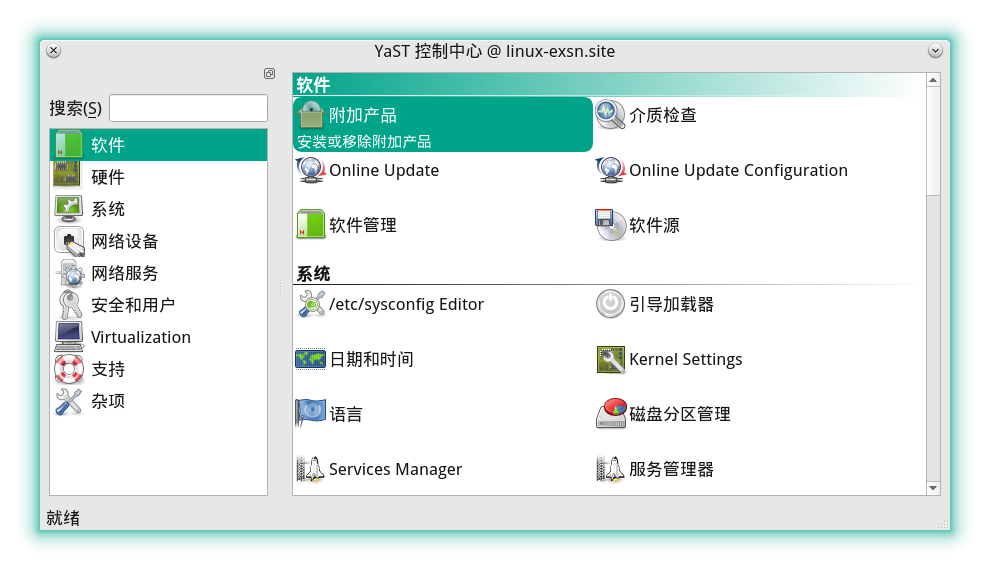
\includegraphics[width=\textwidth]{./pic/yast.png} 
\caption{YaST}\label{yast}
\end{figure}
\paragraph[软件包搜索与一键安装]{\href{http://software.opensuse.org/packages}{软件包搜索}与一键安装} 在这里你可以搜索你想要的软件包。

\begin{figure}[htb]
\centering
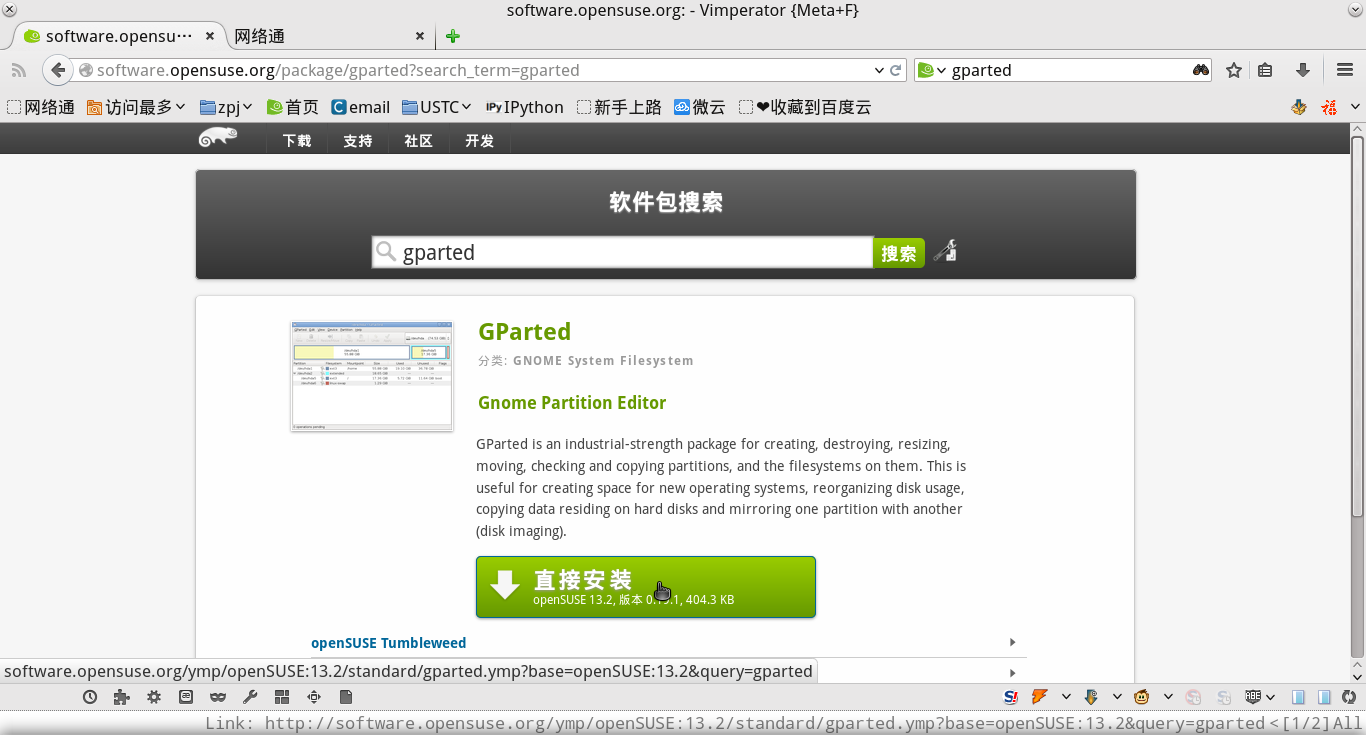
\includegraphics[width=\textwidth]{./pic/software.png} 
\caption{软件包搜索与一键安装}\label{soft}
\end{figure}
与\zy 的区别在于可以找到你的源里面没有的软件。如果你利用\href{https://build.opensuse.org/}{OBS}编译了软件包,那么全世界的人都可以在这里使用它。
火狐浏览器自带了这个搜索引擎。在软件包搜索中找到软件以后,你就可以点击一键安装按钮了。一
键安装使得openSUSE中安装程序十分方便。在你进行软件包搜索后如果有多个源可以选择,同等条件下尽量选择
看起来比较官方的。\[\text{搜索软件}+\text{添加软件源}+\text{刷新软件源}+\text{安装软件}=\text{一条龙服务}\]

\paragraph{常用软件源}\label{repo}

\begin{compactdesc}
 \item[\href{http://mirrors.hust.edu.cn/packman/suse/openSUSE_13.2/}{Packman}]
 提供多媒体编解码器、播放器、Broadcom无线网卡驱动、游戏等
 \item[\href{http://download.opensuse.org/repositories/home:/opensuse_zh/openSUSE_13.2/}{opensuse\_zh}]
 此软件源由中文用户维护,提供WPS等软件。
 \item[\href{http://download.opensuse.org/repositories/KDE:/Extra/openSUSE_13.2/}{KDE:Extra}]
 含有大量额外的KDE程序。
 \item[\href{http://download.opensuse.org/repositories/GNOME:/Apps/openSUSE_13.2/}{GNOME:Apps}]
 含有大量GNOME程序。
 \item[\href{http://dl.google.com/linux/chrome/rpm/stable/i386}{Chrome~32位}|\href{http://dl.google.com/linux/chrome/rpm/stable/x86_64}{64位}] 含有各种稳定版及非稳定版的Google Chrome
\end{compactdesc}
\subsection{KDE下启动程序的方法}
本文所提到的内容一般是任选下列两种方式中的某一种启动。
\paragraph{启动器} 全称Kickoff应用程序启动器,是类似于Windows中“开始菜单”的一个东西,一般可以用Alt+F1调出。新安装的程序可能暂时无法从这里启动。
\begin{figure}[htbp]
\centering
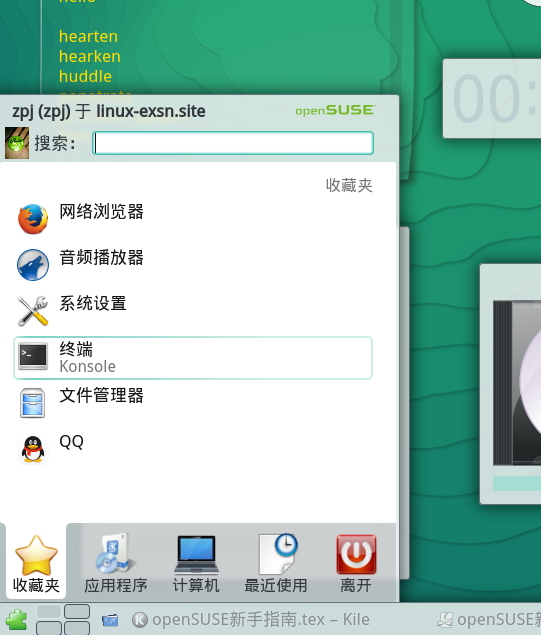
\includegraphics{./pic/kickoff.png} 
\caption{Kickoff应用程序启动器}
\end{figure}
\paragraph{krunner} 是类似于Windows中的“运行”的一个东西,一般可以用Alt+F2调出,之后输入你要运行或要搜索的程序即可。
\begin{figure}[htbp]
\centering
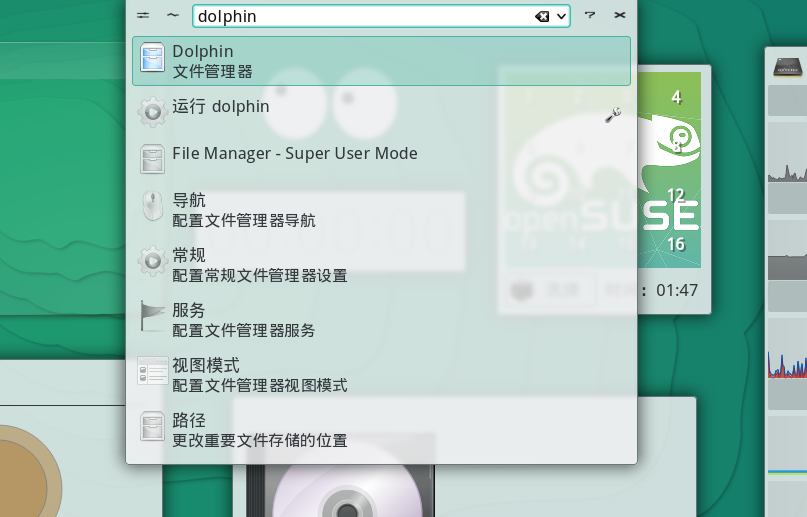
\includegraphics[width=\textwidth]{./pic/krunner.png} 
\caption{krunner}
\end{figure}
\section{更新系统}
为了使你的更新过程尽可能块,你可能需要添加镜像源,比如中国科大镜像,可以参考相
应的\href{https://lug.ustc.edu.cn/wiki/mirrors/help/opensuse}{镜像使用帮助}之
后,按照提示添加并刷新软件源。

之后你就可以在终端中输入\command{sudo zypper up}更新系统了,这是很重要的一步。

运行\zy 进行软件管理时,经常会由于系统后台正在运行一个zypper(系统只能同时运行一个zypper),影响你添加软件源等各种操作。你可以在终端中输入\command{sudo kill pid}把这个进程杀掉,pid是它的进程号。

运行\command{zypper up}的时候常常会遇到以下情况:“将不会安装以下 51 个软件包的更新:blahblahblah”,若对此有疑问请参见\href{https://forum.suse.org.cn/viewtopic.php?t=2777&p=21896}{为什么有些包不会被更新}
\section{中文环境的配置}
用LiveCD安装,无法得到完整的中文KDE环境,所以你需要安装
\begin{Verbatim}[formatcom=\color{codec}]
    kde4-l10n-zh_CN translation-update-zh_CN yast2-trans-zh_CN
\end{Verbatim}

为解决zip压缩包解压后文件名乱码的问题,请安装\soft{unzip-rcc}。

Fcitx是一个中文输入法框架,它对应的包为\soft{fcitx fcitx-config-kde4}。安装好后再启动它,从此你的openSUSE就可以输入中文了。
装好后它的默认词库还很弱,你可以安装一个比较大的词库(非必需)。可%
以参见\href{https://code.google.com/p/hslinuxextra/}{hs\-linux\-extra}以及%
\href{https://www.librehat.com/fcitx-sogou-pinyin-cell-database-convert-import-guide/}{词库教程}%
或者下载我编译好的\href{http://pan.baidu.com/s/1i3HtJ4T}{pyphrase}文件,复制
到家目录的\command{.config/fcitx/pinyin/}中。
\begin{figure}[htbp]
\centering
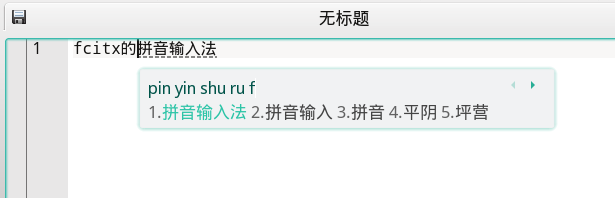
\includegraphics[width=\textwidth]{./pic/fcitx.png} 
\caption{输入法}\label{fcitx}
\end{figure}
当然你也可以不使用默认的拼音输入法而使用Fcitx的谷歌拼音(\soft{goo\-gle\-pin\-yin}),
搜狗拼音(\soft{so\-gou\-pin\-yin})等输入法模块。对于大部分输入法你都可以使用云拼音(\soft{cloud\-pin\-yin})等模块。
安装好云拼音以后,只要在Fcitx的附加组件设置中配置好,你的输入法就可以利用云拼音输入了。注意,某些云拼音来源
可能会失效,如果云拼音无法使用可能就是因为这个原因。
\section[双显卡]{双显卡关闭独立显卡}
\paragraph{NVIDIA} 如果你的显卡支持Bumblebee,请参见\href{https://zh.opensuse.org/SDB:Bumblebee}{SDB:Bumblebee},建议新手加源安装。

\paragraph{AMD} 如果你用的是开源驱动的话,在\command{/etc/init.d/after.local}后面加下面两行,那么开机后将会自动运行以关闭独显:
\begin{Verbatim}[formatcom=\color{codec}]
    echo IGD > /sys/kernel/debug/vgasitcheroo/switch
    echo OFF > /sys/kernel/debug/vgasitcheroo/switch    
\end{Verbatim}
具体请参考\href{https://linuxtoy.org/archives/how-to-use-vga-switcheroo-disable-video-card-linux-kms.html}{关闭独立显卡}。需要注意的是openSUSE并没有\command{/etc/rc.local}文件!你应该用类似于前述的\command{after.local}的文件代替。
\chapter{各种应用}
介绍Linux下面常用的各类程序。本章用到且OBS中没有的软件源一般写在\ref{repo}中。
\section{Linux下的QQ}
腾讯官方提供的QQ for Linux早就无法使用了。webQQ已经挂了,SmartQQ基本半残,只能发送文字——总之很多方法都已经不行了。
但是Chrome和Chromium目前可以运行某些安卓程序,经过测试手机QQ2011可以成功在上面运行。
具体可以参考\href{http://huodong.ustc.edu.cn/Crx}{apk2crx}。
\section{影音播放}
\emp{首先请安装好\href{https://lug.ustc.edu.cn/sites/opensuse-guide/codecs.php}{解码器},否则某些格式将无法播放!}安装解码器等的时候,可能会遇到依赖关系导致的冲突的问题。
冲突的解决请参见\href{https://forum.suse.org.cn/viewtopic.php?t=2867&p=22491#p22491}{安装软件碰到冲突,应该如何选择解决方式?}执行完这一步你的Packman源
就应该添加好了,如果你认为这个源太慢,请尝
试Packman的\href{http://packman.links2linux.org/mirrors}{镜%
像源}
\begin{compactdesc}
 \item[电影] \soft{smplayer},或者\soft{vlc}。
 \item[音乐] 默认的\soft{amarok}与KDE环境集成较好。或者\soft{deepin-music},它启用\href{https://forum.suse.org.cn/viewtopic.php?f=7&t=2530}{百度插件}后便能够下载歌曲了。
\end{compactdesc}
\section{浏览器}
openSUSE下面默认装有Firefox浏览器,它可以通过安装附加组件来增强其功能。

Firefox:默认安装

Chrome:添加Chrome的源后再搜索\soft{chrome}后安装相应的包即可。

Chromium:添加Packman源后再:
\begin{Verbatim}[formatcom=\color{codec}]
    sudo zypper in chromium chromium-ffmpeg chromium-pepper-flash
\end{Verbatim}
即可安装好Chromium
\section{图像处理}
点阵图:\soft{gimp}

矢量图:\soft{inkscape}
\section{办公程序}
\TeX :推荐Kile作为前端,这种情况下你只需要
\begin{Verbatim}[formatcom=\color{codec}]
    sudo zypper in kile texlive-ctex texlive-savesym
\end{Verbatim}
更详细的配置过程请参
考\LaTeX 的\href{https://forum.suse.org.cn/viewtopic.php?f=6&t=2392&p=18750}{配置指南}。除此之外你还可
以用\TeX studio, \TeX works等各种IDE,当然VIM和Emacs这类通用编辑器也是可以的,只不过可能比较难配置。本
文就是用\LaTeX排版的,怎么样,效果还不错吧。

Office:LibreOffice、永中Office或WPS。安装好WPS后需要下载\href{http://pan.baidu.com/s/1ntMEU2P}{Symbols}字体并安装之。否则无法显示各种数学符号等。另外由于WPS是32位的程序,所以如果你是64位操作系统请额外安装\soft{cups-libs-32bit},否则WPS无法输出文档为pdf。
\begin{figure}[htbp]
\centering
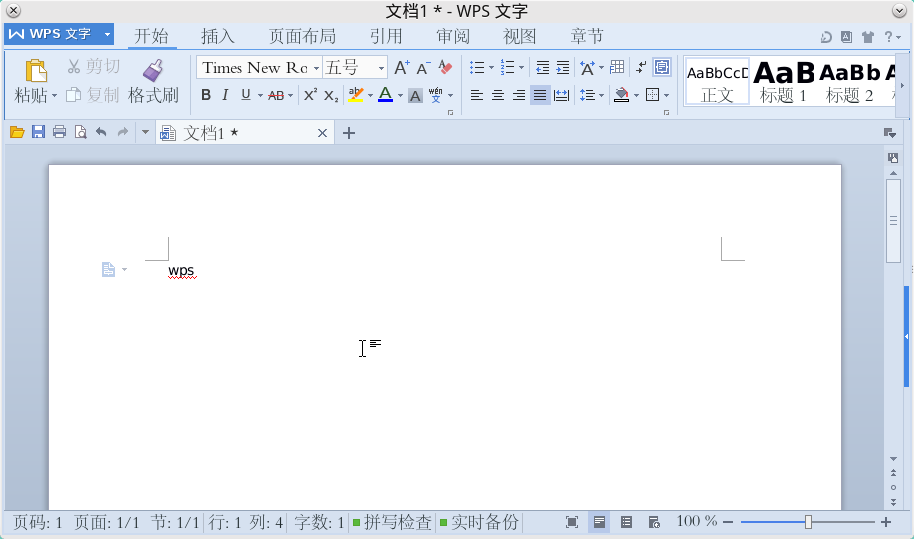
\includegraphics[width=\textwidth]{./pic/wps.png} 
\caption{WPS}\label{wps}
\end{figure}
邮件客户端:\soft{thunderbird}, \soft{kmail}

文本编辑器:Kate, VIM, Emacs etc.
\section{教育程序}
词典:推荐\soft{GoldenDict}\footnote{请务必安装版本号大于1.5的版本或dev版本,否则无法读取.mdx格式},词典请上\href{http://pdawiki.com/forum/forum.php}{pdawiki}下载,
为了让你的词典更聪明,请下载\href{https://zpj.blog.ustc.edu.cn/wp-content/uploads/2014/02/wordsrule.tar.gz}{构词法}。
\begin{figure}[htbp]
\centering
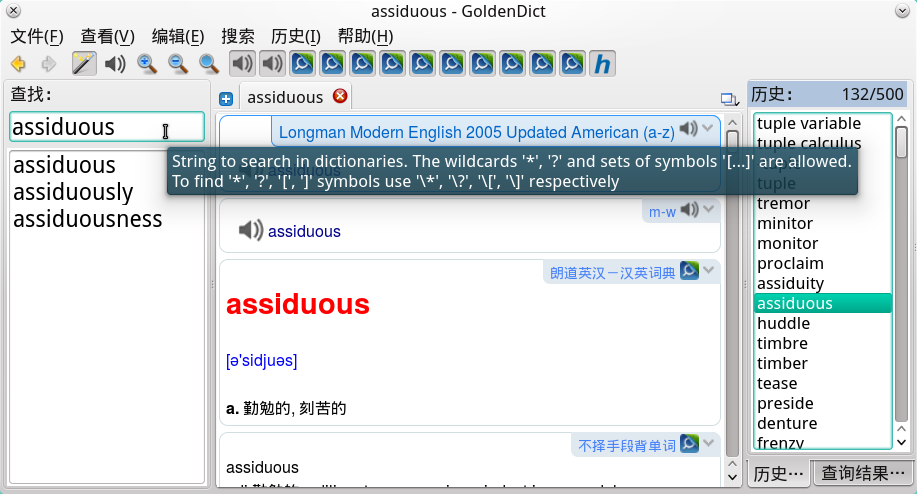
\includegraphics[width=\textwidth]{./pic/goldendict.png} 
\caption{Goldendict}\label{goldendict}
\end{figure}
科学计算、数据处理:\soft{octave}、\textsc{Matlab}、Mathematica、\soft{maxima}、R(\soft{R-base})
\section{网盘}
\begin{compactitem}
 \item 坚果云\soft{nutstore}
 \item 百度云在openSUSE下有非官方的\soft{bcloud}客户端
 \item Dropbox
 \item Wuala
 \item etc.欢迎补充
\end{compactitem}

\section{下载程序}
\begin{compactdesc}
 \item[普通下载] KGet, Firefox的Down\-them\-all!插件,或者直接使用浏览器
 \item[BT] KTorrent, Deluge, Transmition
 \item[ed2k] aMule
\end{compactdesc}

大部分下载都可以用百度网盘这个神器离线下载好,然后再下载到本地。利用有一份田网友的\href{http://git.oschina.net/youyifentian/dupanlink}{百度网盘助手}脚本可以显示百度网盘文件的直接链接。(不过这个助手有时候可能会失效)
\chapter{KDE桌面环境的一些配置}
KDE桌面环境中通过系统设置以及应用程序的设置可以极大的进行自定义,从而提高工作效率。
\section{系统设置}
\subsection{字体设置与管理}
正式文档排版一般都需要宋体、黑体、仿宋、楷体这些字体,从\href{http://pan.baidu.com/s/1mgiHWmO}{百度云}下载好后点击即可安装。开源字体如Ubuntu字体(\soft{ubuntu-fonts})和文泉驿微米黑(\soft{wqy-microhei-fonts})等则可以直接在源中找到甚至默认已经安装好了。

对于非root程序,在\menu{应用程序外观}\me\menu{字体设置}中,你可以调节各种字体字号,当然对于屏幕显示字体最好选择无衬线字体,如Droid Sans Fallback、各种黑体。图\ref{myfont}就是我的相关字体设置。
\begin{figure}[htbp]
 \centering
 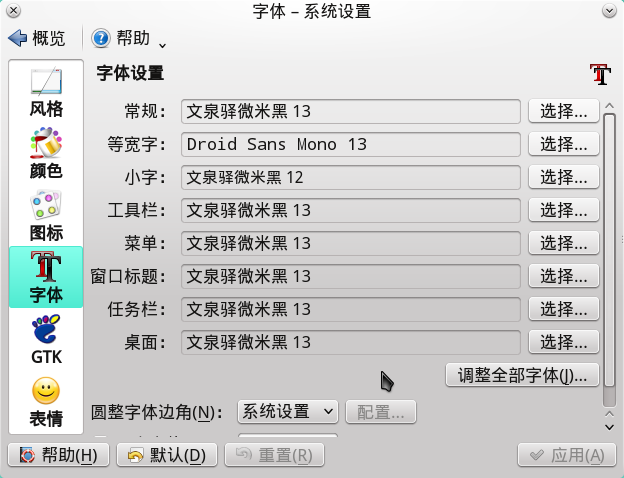
\includegraphics[width=\textwidth]{./pic/fontsettings.png}
 \caption{我的字体设置}\label{myfont}
\end{figure}

对于root程序的字体,你需要在Konsole中以root运行\command{systemsettings}再单独设置。再次强调,在openSUSE中为了能够以root运行相关图形程序,需要使用\command{kdesu}来代替\command{sudo}。

\subsection{桌面效果设置}
在\menu{桌面效果}\me\menu{全部效果}中可以启用各种桌面特效,如模糊效果、半透明效果、桌面立方效果和屏幕反色等功能。

注意,过多的效果可能导致运行缓慢,如果您觉得您的电脑运行缓慢请关闭某些特效。
\subsection{开机自启动管理}
在\menu{开机和关机}\me\menu{自动启动}中可以管理你的启动项。

在\menu{开机和关机}\me\menu{会话管理}中可以关掉或者打开开机时恢复上一次会话。如果你选择打开,那么上次注销或关机时没有关闭的程序在下次登录后会被启动。但这样显然就拖慢了开机速度。
\subsection{快捷方式和手势}
在\menu{快捷方式和手势}\me\menu{自定义快捷键}中你可以为程序或命令设置相应的快捷键,这样你就可以抛弃桌面图标了——所有常用的程序通过快捷键启动,非常用的程序用启动器或Krunner启动。

在\menu{快捷方式和手势}\me\menu{标准键盘快捷键}中你可以设置KDE程序内通用的快捷键,如查找、上一页、第一页、保存、退出等。

在\menu{快捷方式和手势}\me\menu{全局键盘快捷键}中你可以设置各种KDE组件的快捷键。例如在KWin中设置好切换桌面与窗口的快捷键你就可以切换起来如鱼得水。例如我的切换桌面到上下左右采用的是类似于Vim的Ctrl+Alt+k/j/h/l。这一切你都可以自由定制。

KDE默认的截图快捷键是PrtSc,它会调用ksnapshot截图工具。
\subsection{外观设置}
在工作空间外观或者应用程序外观中可以调节相应的外观。

例如在\menu{工作空间外观}\me\menu{窗口装饰}\me\menu{配置按钮}中你可以调整标题栏按钮的位置。我自己采取左关右小的设置可以使关闭和最小化全屏应用程序极为方便,而最大化及恢复只需双击标题栏即可。

\begin{figure}[htbp]
 \centering
 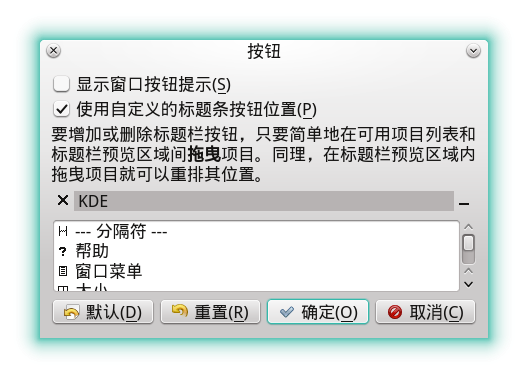
\includegraphics{./pic/botton.png}
 \caption{配置按钮}\label{botton}
\end{figure}
另外很多主题都可以在kde-look上下载或者通过获得新装饰获得。
\subsection{活动、桌面与Plasma桌面挂件}
活动是比桌面大的一个层次,每个活动可以有自己的桌面。而桌面挂件就是一些放在面板或者桌面上的小工具。

桌面空白处右键菜单中选择活动就可以管理活动。另外你可以通过Meta+Tab切换活动。
\begin{figure}[htb]
\centering
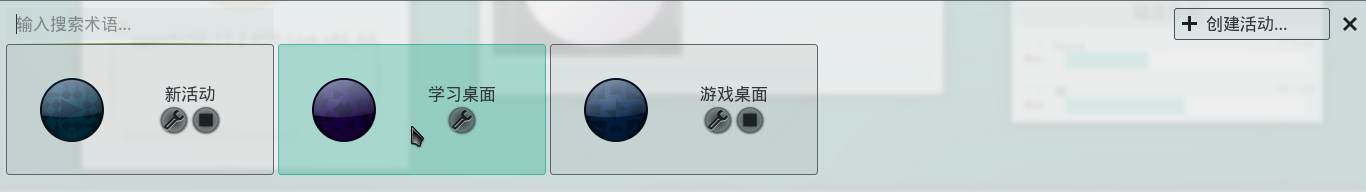
\includegraphics[width=\textwidth]{./pic/activity.png} 
\caption{活动管理}\label{activity}
\end{figure}

按Ctrl+F$i(i=1234\ldots)$可以切换到对应桌面。对应虚拟桌面的一些选项你可以在\menu{工作空间行为}\me\menu{虚拟桌面}中进行设置。对于某个活动中的一组桌面有很多类型可选。在桌面空白处右键菜单中选择桌面设置后你可以选择切换各种布局类型(例如桌面图标就和Windows如出一辙)以及切换壁纸等。
\begin{figure}[htb]
\centering
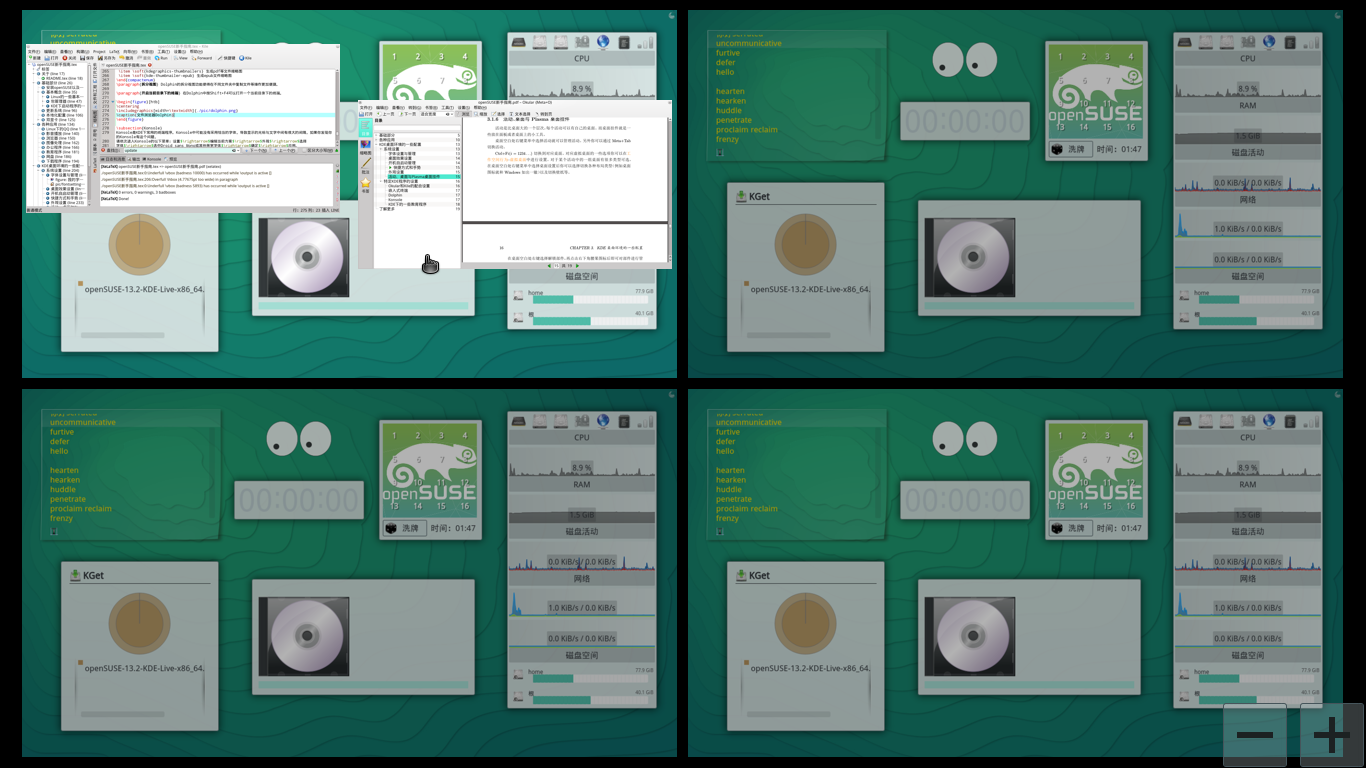
\includegraphics[width=\textwidth]{./pic/virtualdesk.png} 
\caption{多个虚拟桌面}\label{multidesk}
\end{figure}
在桌面空白处右键选择解锁部件,再点击右下角腰果图标后即可对部件进行管理。例如安装好\soft{redshift}及\soft{plasmoid-redshift}挂件后使你能够方便的调节屏幕色温,保护视力(你也可以让它隐藏在任务栏旁边的图标里)。
添加部件时你既可以双击添加到面板,也可以托拽到桌面去。
\begin{figure}[htb]
\centering
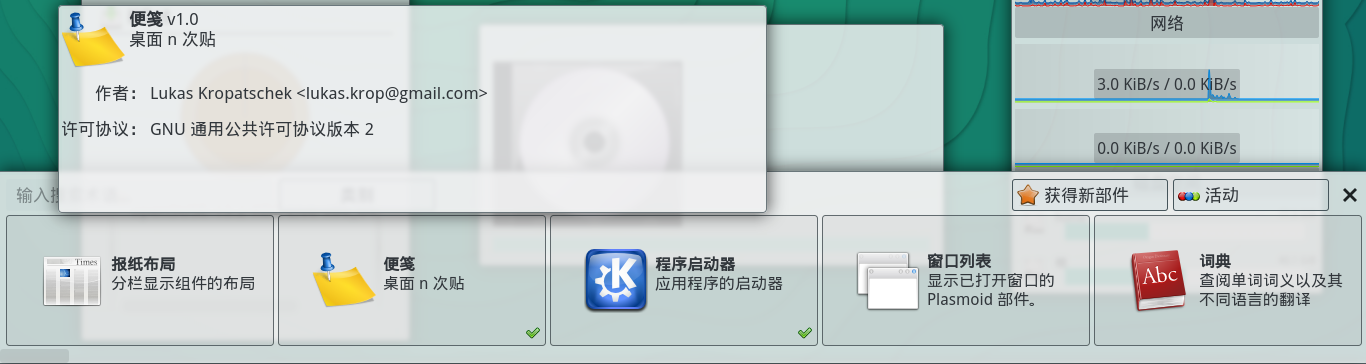
\includegraphics[width=\textwidth]{./pic/plasma.png} 
\caption{添加桌面小挂件}\label{plasma}
\end{figure}

\begin{figure}[htb]
 \centering
 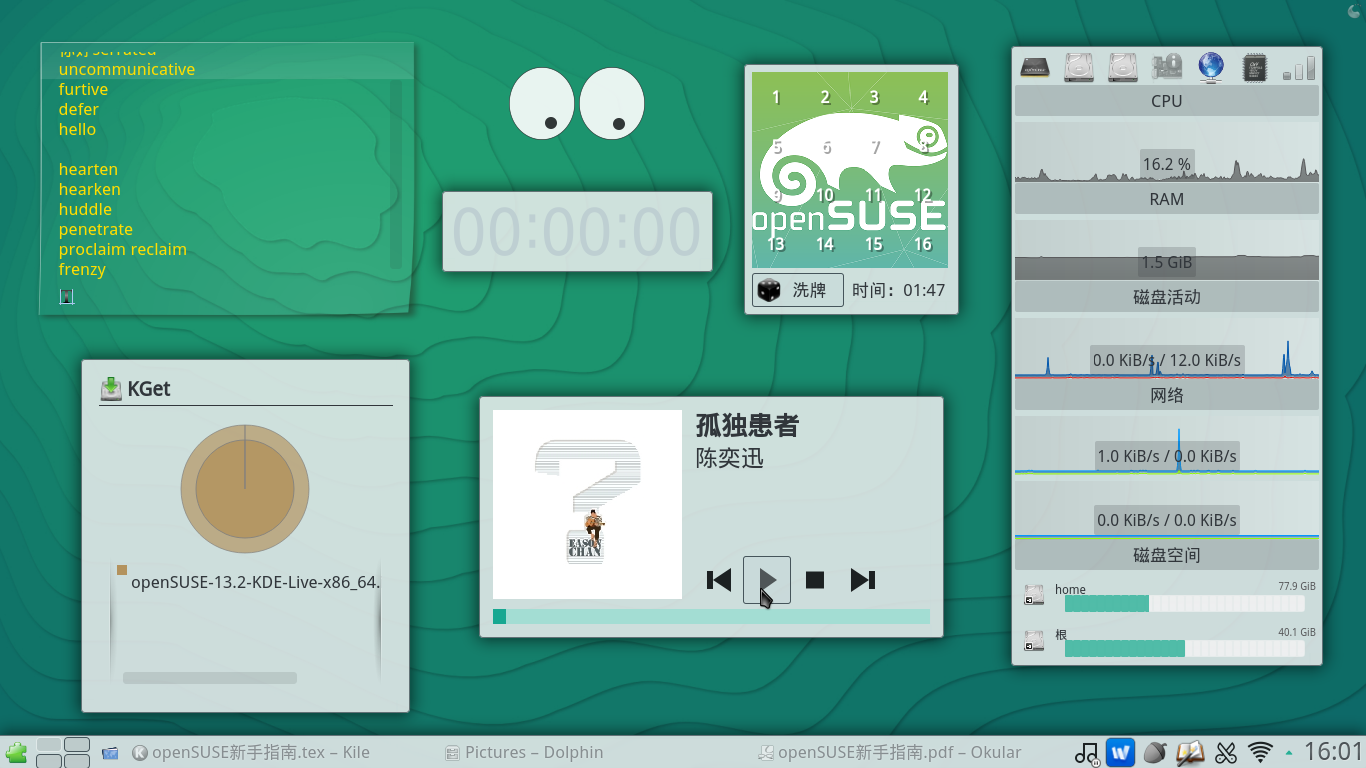
\includegraphics[width=\textwidth]{./pic/desktop.png}
 \caption{我的桌面}\label{mydesk}
\end{figure}

\section{特定KDE程序的设置}
基本所有的KDE程序都可以进行详细的配置,比如工具栏等。在工具栏中添加好常用的图标可以让你每次用的时候都少点几次鼠标。
\subsection{Okular和Kile的配合设置}
编写\LaTeX文档时常用Okular作为pdf阅读器,Kile等作为编辑器。\href{http://zpj.blog.ustc.edu.cn/?p=338}{这里}介绍了Kile与Okular的正反向搜索设置。

\subsection{嵌入式终端}
在Kile中点击右下侧的消息栏上的\menu{Konsole}即出现嵌入式终端。

Dolphin中按F4即可启用/退出嵌入式终端。

Kate中可以启用终端工具视图插件,之后设置好相应快捷键或者启用侧边栏即可方便的启用嵌入式终端。
\subsection{Dolphin}
Dolphin是KDE下默认的文件浏览器,按Ctrl+M可以显示菜单栏,不然就是中看不中用的典型。
\begin{figure}[htb]
\centering
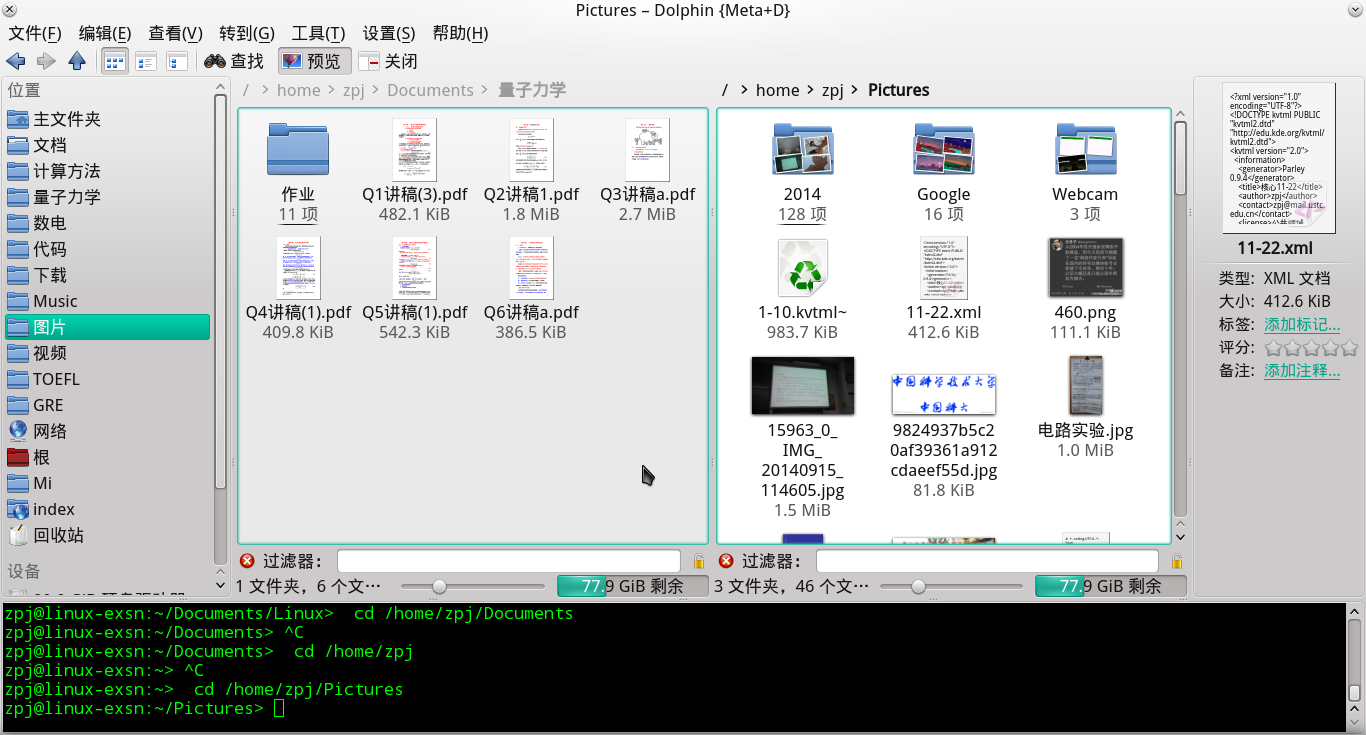
\includegraphics[width=\textwidth]{./pic/dolphin.png} 
\caption{Dolphin的拆分视图以及嵌入式终端}
\end{figure}
\paragraph{Dolphin中的缩略图} Dolphin可以开启缩略图功能,在配置菜单的常规中的预览中选中相应条目即可。如果没有你想要的条目比如pdf,那么你可以用thumbnail为关键字,搜索源中相应的软件包并安装即可。比如:
\begin{compactenum}
 \item \soft{kffmpegthumbnailer} 生成视频文件缩略图
 \item \soft{kdegraphics-thumbnailers} 生成pdf等文件缩略图
 \item \soft{kde-thumbnailer-epub} 生成epub文件缩略图
\end{compactenum}
\paragraph{拆分视图} Dolphin的拆分视图功能使得在不同文件夹中复制文件等操作更加便捷。

\paragraph{开启当前目录下的终端} 在Dolphin中按Shift+F4可以打开一个当前目录下的终端。


\subsection{Konsole}
Konsole是KDE下常用的终端程序。Konsole中可能没有采用恰当的字体,导致显示的光标与文字中间有很大的间隔,如果你发现你的Konsole有这个问题,
请依次进入Konsole的以下菜单:\menu{设置}\me\menu{编辑当前方案}\me\menu{外观}\me\menu{选择
字体}\me选中Droid sans Mono或其他等宽字体\me确定并应用。

在Konsole的编辑配置方案中你可以选择不同的颜色方案等,适用于不同环境。你甚至可以在管理配置方案中为每个方案单独设置一个快捷键。
\subsection{KDE下的一些其他程序}
Parley是一个背单词的程序,可以参考我对它的\href{http://zpj.blog.ustc.edu.cn/?p=294}{介绍}。

KTouch是一个练习打字的程序。

Klipper是一个剪贴板工具,可以生成二维码。

Akregator是一个本地RSS客户端。
\chapter{了解更多}
\begin{compactitem}
 \item \href{https://lug.ustc.edu.cn/sites/opensuse-guide/}{非官方指南}详细的介绍了一些简单的内容
 \item 有问题可以搜索\href{https://zh.opensuse.org/%E9%A6%96%E9%A1%B5}{openSUSE中文维基}
 \item \href{https://forum.suse.org.cn/}{openSUSE中文论坛}
 \item 自学Shell脚本语言,可以参考入门书籍TLCL:\href{http://home.ustc.edu.cn/~zpj/doc/Linux/The_Linux_Command_Line.pdf}{英文版}或\href{http://home.ustc.edu.cn/~zpj/doc/Linux/The_Linux_Command_Line(%e4%b8%ad%e6%96%87%e7%89%88).pdf}{中文版}
 \item 学习\soft{git},有电子书:\href{http://git-scm.com/book/}{英文版HTML}或中文版\href{http://git-scm.com/book/zh}{HTML}/\href{http://liam0205.me/attachment/Git/progit.zh.pdf}{pdf}
\end{compactitem}
\listoffigures
\end{document}
